\documentclass{article}
\usepackage{graphicx}
\usepackage[margin=1in]{geometry}
\usepackage{titlesec}
\usepackage{hyperref} % Add this line for hyperlink support

\titleformat{\section}{\large\bfseries}{\thesection}{.8em}{}
\titlespacing*{\section}{0pt}{1.5ex plus 1ex minus .2ex}{0.5ex plus .2ex}

\title{Self-Evaluation}
\author{Aaron Fulton}
\date{\today}

\begin{document}

\maketitle
\newpage

\section{Page Appearance in Different Web Browsers}
\label{sec:page-appearance} 

\textbf{Browsers tested:}
\begin{itemize}
    \item Brave (Chromium-based browser)
    \item Firefox
    \item Safari (on mobile) 
\end{itemize}

\textbf{Comparison:}
\begin{itemize}
    \item \textbf{Brave:} The page appeared as expected, since it was designed using Brave and the Live Server extension for VS Code.
    \item \textbf{Firefox:} Firefox displayed the page similarly to Brave, with no observable differences.
    \item \textbf{Safari:} The page was made responsive and displays well on mobile, but there is a minor issue with text 
    elements not being fully readable due to overflow when switching to a horizontal view.
\end{itemize}

\textbf{Conclusion:} The page works well on all desktop browsers tested, with minor issues observed on mobile.

\section{Link Functionality}
\label{sec:link-functionality} 

\textbf{Test Summary:}
All links were tested, and 5 of 5 links worked correctly.

\section{HTML and CSS Validation Results}
\label{sec:validation-results} 

\subsection{HTML Validation}
\textbf{Validation Tool:} \texttt{https://validator.w3.org}

\textbf{Result:}
\begin{figure}[h]
    \centering
    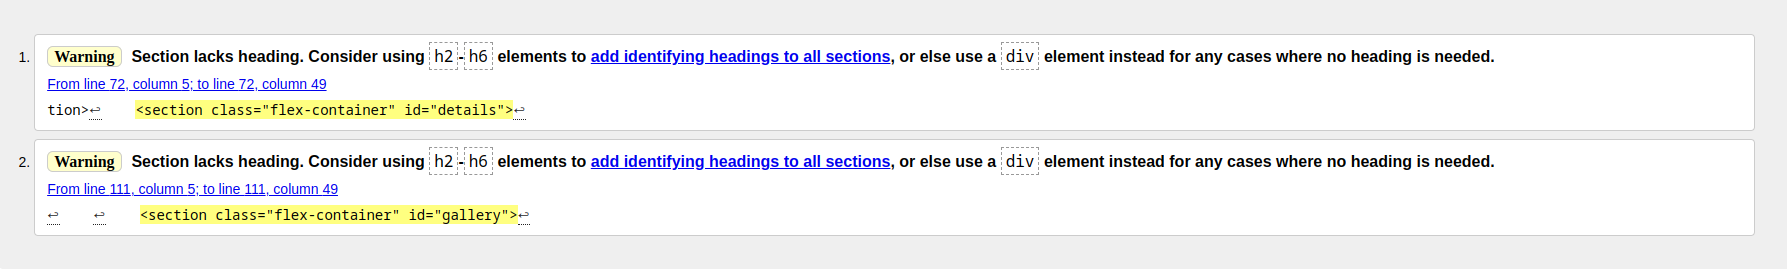
\includegraphics[width=0.5\textwidth]{graphics/HTML_validation.png}
    \caption{HTML Validation Results}
\end{figure}

\textbf{Summary:} The HTML is valid.
\begin{itemize}
    \item Warnings: There were 2 small warnings about the lack of usage of \texttt{h1..h6} tags after the \texttt{article} tag.
\end{itemize}

\subsection{CSS Validation}
\textbf{Validation Tool:} \texttt{https://jigsaw.w3.org/css-validator}

\textbf{Result:}
\begin{figure}[h]
    \centering
    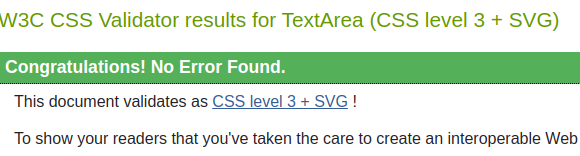
\includegraphics[width=0.5\textwidth]{graphics/CSS_validation.png}
    \caption{CSS Validation Results}
\end{figure}

\textbf{Summary:} The CSS is valid.

\section{Final Remarks}
\label{sec:final-remarks} 

\textbf{Overall:} The page worked well on several browsers of different sizes and met the requirements of the assignment. 
While my goal was to create a page with more responsive features including a dark mode theme and a mobile-friendly layout 
this was a partial success in my eyes but there is definitely there is still room for improvement.

\end{document}
